Dieser Versuch befasst sich mit der Messung der Wirk- und Blindleistung mithilfe eines Multiplikators und eines trägen Messgerätes. Es wird zusätzlich die Scheinleistung berechnet, und die berechneten und gemessenen Ergebnisse werden miteinander verglichen.

\subsubsection{Versuchsaufbau}

Der Versuchsaufbau ähnelt weitestgehend dem Aufbau aus dem in Abschnit \ref{sec:Aufbau2.2.1} beschriebenen. Es wird jedoch das Oszilloskop durch einen Multiplikator und ein träges, analoges Messgerät gemäß Abbildung \ref{fig:Plan2-2} ersetzt. Das Messgerät wird auf Gleichspannung eingestellt und misst somit den Gleichanteil der Spannung $u_P(t)$, welche durch die Multiplikation von Spannung $u_U(t)$ und zum Strom proportionalen Spannung $u_I(t)$ eine zur Momentanleistung proportionale Größe dar stellt. Somit kann durch Bestimmung des Proportionalitätsfaktors die Wirkleistung bestimmt werden.

\begin{figure}[H]
\centering
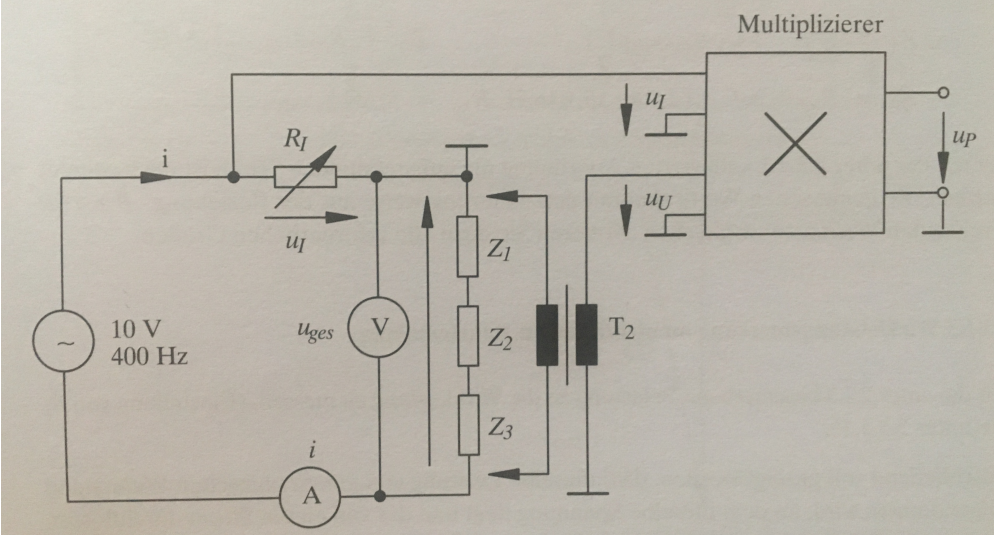
\includegraphics[width=0.7\linewidth]{Images/Aufbau2-2.png}
\caption{Schaltplan eines Versuches zur Messung der Wirkleistung eines Schaltkreises}
\label{fig:Plan2-2}
\end{figure}

Die Impedanzen werden je nach zu messender Größe verändert, und im folgenden genauer erläutert.

\subsubsection{Kalibrierung des Drehspulmessinstrumentes}

